\section{Purpose}
\subsection{General Purpose}

The main scope of this document is to define requirements for the application development, in order to make a correct project planification.
\par
To do this, we will analyze:

\begin{itemize}
\item system;
\item functional and unfunctional requirements;
\item constraints;
\item relationships between stakeholders;
\item possible scenarios and tests;
\end{itemize}
\bigskip
These will be shown using different languages such as Alloy and UML.
Then, we will define the context in which our application will be developed.\\
During Sars-Cov-2 emergency, several countries imposed the lockdown in order to hinter the virus diffusion.
People had to change their habits, in fact they could go out only for necessary needs, such as going to the market or pharmacy.\\
For instance people must pay attention while they're entering in the market due to the long queue, which could increase the possibility of virus diffusion.
This fact obliged people to stay for a long time standing up and waiting their turn losing a lots of time. 
\pagebreak

\subsection{Goals}

This are the goals:

\begin{description}
    \item[G1]User enters once arrived at the market.
    \item[G2]Put a limit to the number of Users in the market.
    \item[G3]Smart User can make a Reservation of a seat in the market's queue.
    \item[G4]Smart User can book in advance a Visit in the market.
    \item[G5]Mobile User can make a Reservation of a seat in the market's queue.
    \item[G6]Mobile User can book in advance a Visit in the market.
    \item[G7]Smart User can cancel a booking which can be either a Visit or a Reservation.
    \item[G8]Mobile User can cancel a booking which can be either a Visit or a Reservation.
\end{description}


 
\section{Scope}

The aim of the project is to develop an application which, thanks to an intuitive interface, will avoid customers waiting outside the market.
In order to do that, we offer customers three grocery shopping option: 

\begin{itemize}
\item \textbf{Visit}: it's a planned appointment with given date and range time;
\item \textbf{Reservation}: it consits in reserving a virtual seat in market's queue;
\item \textbf{Direct Entrance}: it allows aged customers to enter without any bookings;
\end{itemize}
\bigskip
The main options shown in this documents are the first two in order to avoid customers to line up outside the market. Those are avaiable only for \textbf{Smart} and \textbf{Mobile Users} (their definitions are in subsection 1.3.1).\par
In particular, in order to avoid waiting in line, Users will be allerted by \textbf{notifications} (Smart Users) or a \textbf{SMS} (Mobile Users). These inform them about his time schedule required to reach the market in time.
Only for Smart User the application will provide the position in queue and the time to reach the market.\par
An alphanueric string will be provided to Mobile Users for going in and out from the market. This string for Smart User is converted in two-dimensional bar code using the standard QRCode. This must be submitted at the entry of the market.\par
Instead, the third option is only avaiable if an user is older than 65 years old, but with limitations. For instance they can go grocery shopping only in certain days and timeslots. \\
In particular, the Direct Entrance is avaiable only from Monday to Friday in the range time between 9.00 A.M and 13.00 P.M. The reason for this selection is due the fact that in this ranges there are fewer customers than any other periods because are working hours. \par
This third option is made especially for aged people who don't have even a mobile phone. \par
The 3 provided methods to go shopping in the market are based on research made by \textit{CENSIS} and \textit{Pew Research Center} that shows how many people in Italy own a smartphone, mobilephone or none.\\
As was shown in these two researches, made in 2018, 71\% of italians own a smartphone, the other 20\% own a mobilephone and the remaining 8\% have none of the two.
Considering that most of the people that don't own a smartphone / mobilephone are older than 65 years old, we can cover most of the customers' market with these 3 shopping options.\\
Analyzing the multiple years data, in the future there will be a significant increase of smartphone/phone and so we cover almost the entire population.\par 
Anyway the RASD document is not focused on the third option.\par


\begin{figure}[H]
  \centering
  %\subfloat[Plot 1.]
  {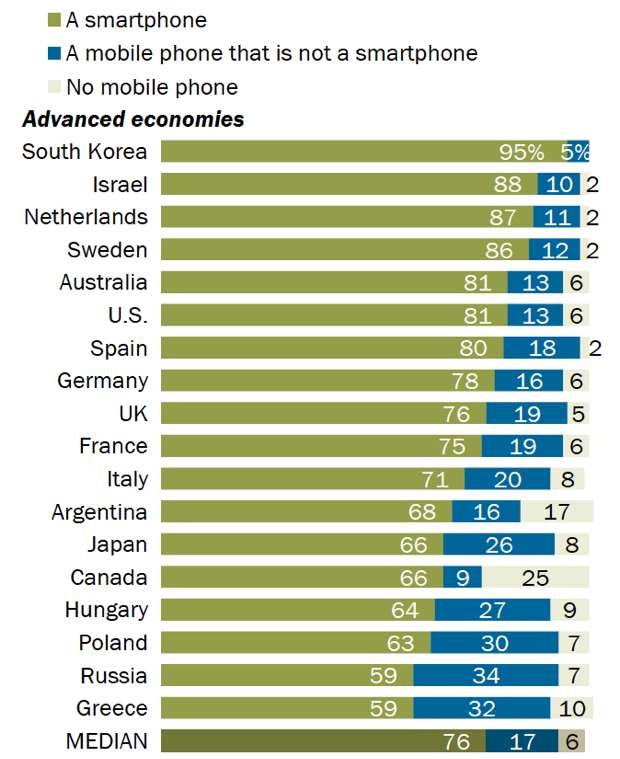
\includegraphics[scale=0.50]{images/statistics_smartphone.png}}
  \hfill
  %\subfloat[Plot 2.]
  {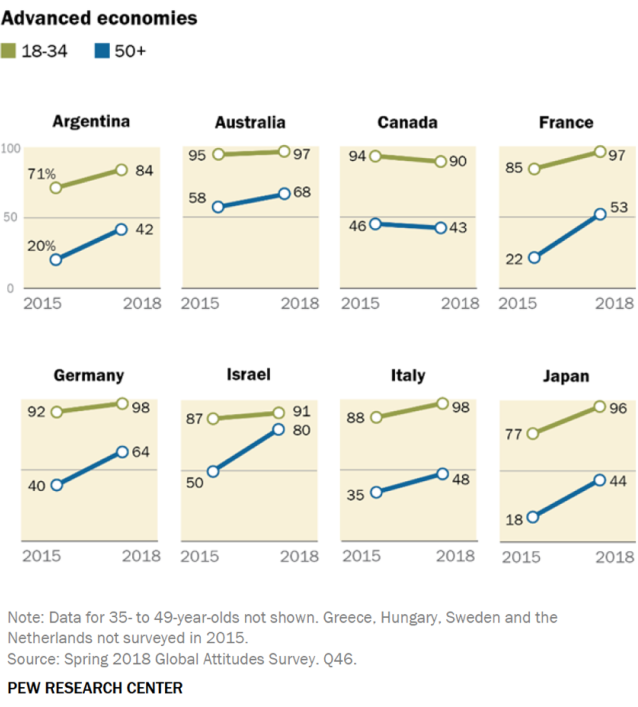
\includegraphics[scale=0.55]{images/statistics_smartphone2.png}\label{fig:f2}}
  \caption{The following charts from Pewresearch website shows percentage of smartphone and mobilephone's owners in each Country.}
\end{figure}

\begin{figure}[H]
  \caption{World and Machine rapresentation.}
  \centering
  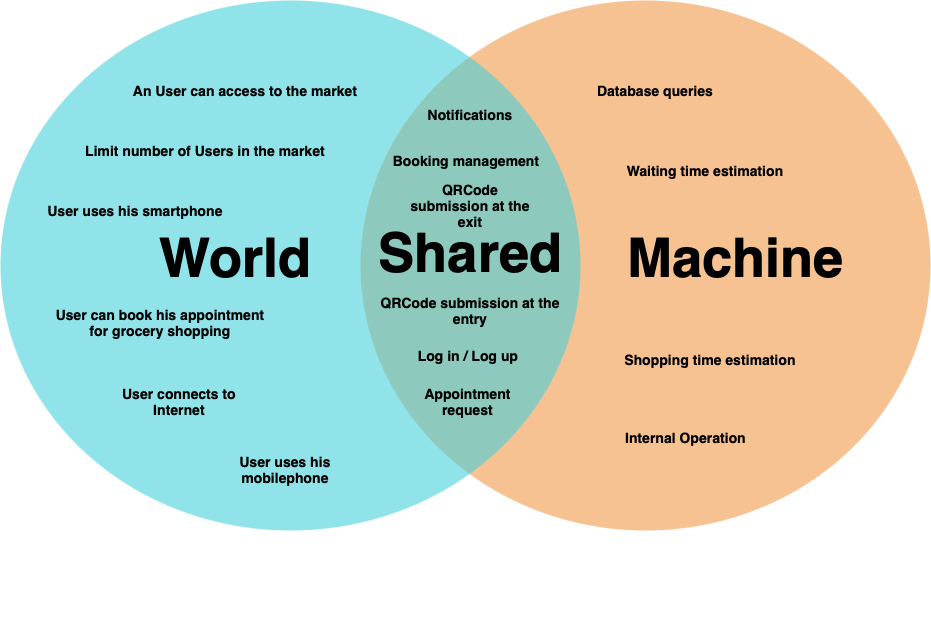
\includegraphics[scale = 0.38]{diagrams/VENN.png}
\end{figure}
\par
\subsection{World}

It represents the environment in which the system is placed. In particular it's composed by events which are affected by the system, but not directly connected with it.
The main \textit{World Phenomena} are:

\begin{itemize}
\item an User can access to the market;
\item limit number of Users in the market;
\item User can book his appointment for grocery shopping;
\item User use his mobilephone / smartphone;
\end{itemize}


\subsection{Machine}
It represents the portion of system to be developed.
The main \textit{Machine Phenomena} are:
\begin{itemize}
\item internal operations;
\item managing any bookings;
\item waiting time estimation;
\item data storage operations;
\end{itemize}
\subsection{Shared Phenomena} 
In this model it needs a common interface to link World and Machine which is composed by the Shared phenomena. \\
Graphically is represent by an intersection between the World and the Machine. In this way World and Machine phenomena are observed from each other.  
The main application Shared Phenomena are the following:
\begin{itemize}
\item Notifications;
\item sign in / sign up;
\item Booking management;
\item QRCode submission;
\item appointment request;
\end{itemize}

\bigskip
\section{Definitions, Acronyms, Abbreviations}
\subsection{Definitions}
\label{info}
\begin{itemize}
\item \textbf{User}: Generic customer who plan to shop in the market. He/she could be a Smart or Mobile User;
\item \textbf{Smart User}: User who has got a smartphone with CLup app. She/He's able to manage bookings by herself/himself;
\item \textbf{Mobile User}: User who hasn't got a smartphone (only mobilephone) and so he's not able to manage Booking by himself. A Mobile User allows a Receptionist to manage his booking by calling a telephone number by interacting with him;
\item \textbf{CLup Operator}: desktop application used by Receptionists to manage bookings of Mobile Users;
\item \textbf{Shopping Size}: it's the size of the grocery shopping. It could be \textit{small}, \textit{medium}, \textit{large} depending on the number of items that users will buy. The duration of the permanence inside the market is based on it; 
\item \textbf{Booking}: it indicates the generic appointment of a User in the market. It could be a Reservation or a Visit;
\item \textbf{Reservation}: it's a type of booking. Users simply book a seat at the market's queue. In addition User have to indicate the Shopping Size; 
\item \textbf{Visit}: it's a Booking planned in advance by Users. It is planned by putting the date and the range time in which the User is going grocery shopping. In addition User have to indicate the Shopping Size; 
\item \textbf{Reader}: it reads QRCode at the market's entrance. It allows User to go in / out;
\item \textbf{Booking submitted}: it means that the QRCode related to it is already submitted in the Reader;
\item \textbf{Visit activated}: it's a Visit which already booked but not yet submitted by the User;
\item \textbf{Reservation activated}: it's a Reservation which already booked but not yet submitted by the User;
\item \textbf{Timestamp}: a digital record of the time of occurrence of a particular event;
\item\textbf{Mirroring}: Mirroring is a technique to allow server to automatically maintain a dual backup of the system;
\end{itemize}

\subsection{Acronyms}
\begin{itemize}
\item \textbf{RASD}: Requirement Analysis and Specification Document;
\item \textbf{HW}: Hardware;
\item \textbf{SW}: Hardware;
\item \textbf{API}: Application Programming Interface;
\item \textbf{HTTPS}: Hypertext Transfer Protocol Secure;
\item \textbf{DBMS}: Database Management System;
\item \textbf{FOL}: First Order Logic;
\item \textbf{UML}: Unified Modeling Language;
\end{itemize}
\medskip
\subsection{Abbreviations}
\begin{itemize}
\item \textbf{App}: Application;
\item \textbf{Gn}: n-th goal;
\item \textbf{Rn}: n-th requirement;
\end{itemize}



\section{Revision history}
\begin{itemize}
\item \textit{Version 1.0} (11 December 2020);
\item \textit{Version 1.1} (20 December 2020): fixed errors and layout; 
\end{itemize}

\pagebreak
\section{Reference Documents}
This document is strictly based on:
\begin{itemize}
\item The specification of the \textbf{RASD and DD assignment} of the Software Engineering II course, held by professor Matteo Rossi and Elisabetta Di Nitto at the Politecnico di Milano, A.Y 2020/2021;
\item \textbf{Slides} of Software Engineering 2 course on BEEP;
\end{itemize}
\section{Document Structure}
Mainly the current document is divided in 4 chapters, which are:
\begin{itemize}
\item[1]\textbf{Introduction}: it aims to describe the environment and the demands taken into account for this project. In particular it's focused on the reasons and the goals that are going to be achieved with its development;
\item[2]\textbf{Overall Description}: it's a high-level description of the system by focusing on the shared phenomena and the domain model (with its assumption); 
\item[3]\textbf{Specific Requirements}: it describes in very detail the requirements needed to reach the goals. In addition it contains more details useful for developers (i.e information about HW and SW interfaces);
\item[4]\textbf{Formal Analysis}: this section contains a formal description of the main aspect of the World phenomena by using Alloy;
\item[5]\textbf{Effort Spent}: it shows the time spent to realize this document, divided for each section;
\item[6]\textbf{References}: it contains the references to any documents and to the Softwares used in this document.
\end{itemize}

